\documentclass[xcolor=dvipsnames]{beamer}

% Packages
\usepackage{bm}
\usepackage{wasysym}


%% Theme related.
\usetheme{default}
\setbeamerfont{author}{size = \large}
\setbeamerfont{institute}{size=\large}
\setbeamerfont{footline}{series = \bfseries}
\setbeamertemplate{navigation symbols}{}
\setbeamertemplate{frametitle}[default][center]
\setbeamertemplate{itemize items}[circle]
\definecolor{Red}{rgb}{.9,.05,.05}
\setbeamercolor{alerted text}{fg=Red}
\usefonttheme[onlymath]{serif}


%% Math
\newcommand{\Reals}{\mathbb{R}}
\newcommand{\wh}[1]{\widehat{#1}}
\newcommand{\wt}[1]{\widetilde{#1}}
\DeclareMathOperator*{\argmin}{argmin}

%% Font
\newcommand{\red}[1]{\textcolor{red}{#1}}
\newcommand{\blue}[1]{\textcolor{blue}{#1}}

\title{Nonparametric Regression via Graph Laplacian Smoothing}

\author{Alden Green}
\institute{Department of Statistics and Data Science \\

\includegraphics[width=.5 \textwidth]{figures/cmu.png}}
\date{}

\begin{document}
	
\begin{frame}
\titlepage
\end{frame}

\addtobeamertemplate{navigation symbols}{}{
	\usebeamerfont{footline}
	\usebeamercolor[fg]{footline}
	\hspace{1em}
	\insertframenumber
}
\addtocounter{framenumber}{-1}

%%% (1) Introduction
% (A) Method

\begin{frame}{Graph Laplacian smoothing}
We observe: 
\begin{itemize}
	\item Design points $X_1,\ldots,X_n \in \Omega$ (sampled from distribution $P$ supported on $\Omega \subseteq \Reals^D$).
	\item Responses $\vec{Y} = (Y_1,\ldots,Y_n)$.
\end{itemize}
\begin{figure}
	\includegraphics[width=.6\textwidth, trim = {0 3cm 0 1.5cm}]{figures/warmup_example_1.pdf}
\end{figure}
\pause
{\bf Idea}: Solve a penalized least squares problem with penalty involving Laplacian of a neighborhood graph built over the design.
\end{frame}

\begin{frame}[t]{Graph Laplacian smoothing}
Form a {\bf neighborhood graph} $G = (\{X_1,\ldots,X_n\}, W)$. 
\begin{itemize}
	\item Compute adjacency matrix $W$ using kernel $\eta$ and radius $\varepsilon$, so
	\begin{equation*}
	W_{ij} = \eta\biggl(\frac{\|X_i - X_j\|}{\varepsilon}\biggr)
	\end{equation*}
	measures similarity between points $X_i$ and $X_j$. 
	\item E.g. weighted $\varepsilon$-geometric graph: $W_{ij} = 1(\|X_i - X_j\| \leq \varepsilon) \cdot \phi(\|X_i - X_j\|/\varepsilon)$.
\end{itemize}
\pause
\begin{figure}
	\centering
	\includegraphics[width=.6\textwidth, trim = {0 3cm 0 1.5cm}]{figures/warmup_example_2.pdf}
\end{figure}
\end{frame}

\begin{frame}[t]{Graph Laplacian smoothing}
Compute the {\bf Laplacian matrix} $L = D - W$, where 
\begin{equation*}
D_{ii} = \sum_{j = 1}^{n} W_{ij},
\end{equation*}
is the degree of $X_i$ in $G$.
\vspace{.2cm}
\begin{figure}
	\centering
	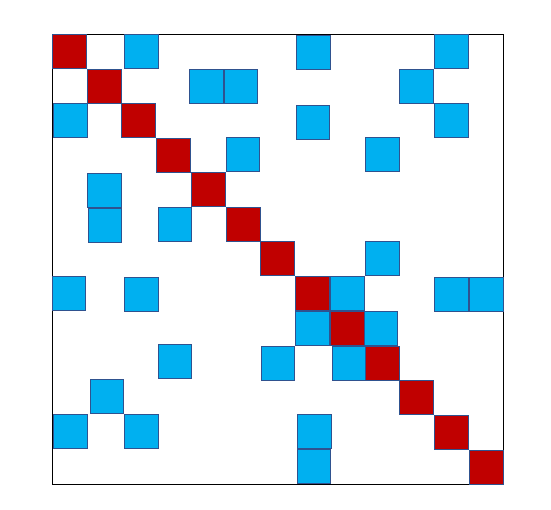
\includegraphics[height=.4\textheight]{figures/laplacian_matrix.png}
\end{figure}
\end{frame}

\begin{frame}[t]{Graph Laplacian smoothing}
Solve the penalized least squares problem
\begin{equation*}
\wh{\theta} := \argmin_{\theta \in \Reals^n} \frac{1}{n}\sum_{i = 1}^{n}(Y_i - \theta_i)^2 + \lambda \theta^{\top} L \theta.
\end{equation*}
{\bf Intuition}: The penalty $\theta^{\top} L \theta = \sum_{i,j = 1}^{n} (\theta_i - \theta_j)^2 W_{ij}$ enforces a notion of smoothness.
\pause
\begin{figure}
	\centering
	\includegraphics[width=.6\textwidth, trim = {0 3cm 0 1.5cm}]{figures/warmup_example_3.pdf}
\end{figure}
\end{frame}

% (C) Motivation
\begin{frame}{Laplacian smoothing: motivation}
Why Laplacian smoothing?
\begin{itemize}
	\item \emph{Computational ease.} Sparse graph, fast solvers.
	\item \emph{Generality.} Makes sense whenever one can form a graph $G$. 
	\item \emph{Weak supervision.} Naturally extends to semi- and unsupervised problems.
\end{itemize}
\pause
Today I will focus on...
\begin{itemize}
	\item \emph{Univariate intuition}. In $1d$, discretization of spline-based estimator.
	\item \emph{Multivariate extension}. Depends in a sensible manner on geometric structure of design.
	\item \emph{Statistically optimal}. Achieves minimax rates over Sobolev classes.
\end{itemize}
\end{frame}

\begin{frame}[t]{Laplacian smoothing: motivation}
In $1d$, recall the first-order~\alert{smoothing spline} estimator
\begin{equation*}
\widetilde{f} := \argmin_{f \in H^1} \|Y - f\|_n^2 + \lambda \int (f')^2.
\end{equation*}
\pause
As $n \to \infty, \varepsilon \to 0$, for smooth functions $f$ (say $f \in C^{1,\alpha}$), 
\begin{equation*}
f^{\top} L f = \frac{1}{2}\sum_{i,j = 1}^{n} \bigl(f(X_i) - f(X_j)\bigr)^2 W_{ij} \approx \int \bigl(f')^2 p^2 .
\end{equation*}
\pause
{\bf Interpretation}: Laplacian smoothing serves as a \alert{discretized} approximation to a~\alert{density-weighted} smoothing spline. 
\begin{itemize}
	\item Density-weighting useful under (hard or soft) cluster assumption, or manifold hypothesis.
	\item Discretization useful when density $p$ is unknown, and for multivariate extension.
\end{itemize}
\end{frame}

% (B) Setup
\begin{frame}{Basic problem setup}

{\bf Nonparametric regression, random design}: We observe $(X_1,Y_1),\ldots,(X_n,Y_n)$, where $X_1,\ldots,X_n \in \Reals^D$ are sampled independently from density $p$, and
\begin{equation*}
Y_i = f_0(X_i) + Z_i, \quad Z_i \sim N(0,1).
\end{equation*}
Goal is to accurately estimate the unknown regression function $f_0$, which is assumed to be first-order \alert{Sobolev} smooth, with semi-norm
\begin{equation*}
|f_0|_{H^1}^2 := \int \|\nabla f_0(x)\|^2 \,dx \leq 1.
\end{equation*}
{\bf Loss}: Measured in \alert{empirical norm}, meaning
\begin{equation*}
\|\wh{\theta} - f_0\|_n^2 = \frac{1}{n}\sum_{i = 1}^{n} \bigl(\wh{\theta}_i - f_0(X_i)\bigr)^2.
\end{equation*}
\end{frame}


% (2) Results

\begin{frame}[t]{Rates of convergence: univariate case}

{\bf Background}: First-order smoothing splines are known to achieve minimax optimal rates of convergence over first-order Sobolev classes.
\begin{equation*}
\sup_{f_0 \in H^1(\Omega)} \mathbb{E}\|\wt{f} - f_0\|_{L^2(\Omega)}^2 \asymp n^{-2/3} \asymp \inf_{\wh{f}}\sup_{f_0 \in H^1(\Omega)} \mathbb{E}\|\wt{f} - f_0\|_{L^2(\Omega)}^2
\end{equation*}

{\bf Question}: Can Laplacian smoothing match this rate of convergence?

\end{frame}

\begin{frame}[t]{Rates of convergence: univariate case}

{\bf Result}: Yes. In fact, Laplacian smoothing matches these rates so long as $\Omega$ has \alert{intrinsic dimension} $d = 1$ (no matter the ambient dimension).
\vspace{.2 in}
\pause

Main idea behind result: 
\begin{itemize}
	\item \alert{Bias-variance} trade off involving eigenvalues $\rho_k(L)$,
	\begin{equation*}
	\|\wh{\theta} - f_0\|_n^2 \lesssim \lambda |f_0|_{H^1}^2 + \sum_{k = 1}^{n}\frac{1}{(1 + \lambda \rho_k(L))^2}.
	\end{equation*}
	\item Under conditions on $\Omega$ and $P$, eigenvalues satisfy \alert{modified Weyl's Law} scaling, $\rho_k(L) \asymp k^{2} \wedge \varepsilon^{-2}$.
	\item Choosing $\varepsilon \asymp (\log n/n)$ and $\lambda \asymp n^{-2/3}$ balances bias and variance.
\end{itemize}
\pause 
{\bf Interpretation}: Laplacian smoothing is a statistically reasonable way to adapt a classic variational scheme (first-order smoothing splines) to complex geometric structures. 
\end{frame}

\begin{frame}[t]{Rates of convergence: multivariate case}

{\bf Background}: Extension of first-order smoothing splines to multivariate setting---replacing derivative by gradient,
\begin{equation*}
\min_{f_0 \in H_1} \|\vec{Y} - f\|_n^2 + \lambda \int \|\nabla f\|^2 \,dx,
\end{equation*}
does not lead to a well-posed method.\pause
\begin{itemize}
	\item \alert{Sobolev embedding theorem}: Convergence in Sobolev norm $\not\Longrightarrow$ pointwise convergence. There exist functions $f_k$ satisfying $f_k(X_i) = Y_i$ yet 
	$$\lim_{k \to \infty} \int \|\nabla f_k\|_2^2 = 0.$$
\end{itemize}
\pause
{\bf Question}: Any hope for Laplacian smoothing?
\end{frame}

\begin{frame}[t]{Rates of convergence: multivariate case}

{\bf Result}: Yes. 
\begin{itemize}
	\item Laplacian smoothing achieves optimal rates of convergence ($n^{-2/(2 + d)}$) so long as $\Omega$ has intrinsic dimension $2 \leq d \leq 4$.
	\item Rate of convergence is $n^{-4/(3d)}$ when $d \geq 5$. Suboptimal.
\end{itemize}
\pause
Main idea behind result: 
\begin{itemize}
	\item Bias-variance tradeoff involving eigenvalues $\rho_k(L)$,
	\begin{equation*}
	\|\wh{\theta} - f_0\|_n^2 \lesssim \lambda |f_0|_{H^1}^2 + \sum_{k = 1}^{n}\frac{1}{(1 + \lambda \rho_k(L))^2}.
	\end{equation*}
	\item Under conditions on $\Omega$ and $P$, eigenvalues satisfy modified Weyl's Law scaling, $\rho_k(L) \asymp k^{2/d} \wedge \varepsilon^{-2}$.
	\item Choosing $\varepsilon \asymp (\log n/n)^{1/d}$ and $\lambda \asymp n^{-2/(2+ d)}$ balances bias and variance when $2 \leq d \leq 4$.
\end{itemize}
\pause
{\bf Interpretation}: ???
\end{frame}

\begin{frame}
\centering
\huge
\blue{Questions}
\end{frame}

% (3) Questions
\begin{frame}[t]{Questions}
\begin{itemize}
	\item Can we situate Laplacian smoothing within the standard regression toolbox?
	\item Is there a conceptually coherent way to extend the estimator to be defined over all of $\Omega$?
\end{itemize}
\textbf{My thought}: Both of these questions are (at least somewhat) related to properties of interpolation.
\end{frame}

% (3A): Equivalent kernel
\begin{frame}[t]{Equivalent kernel of Laplacian smoothing}

\textbf{Question 1}: Can we situate Laplacian smoothing within the standard regression toolbox?
\pause

\textbf{Goal}: Recast Laplacian smoothing as approximately the estimate produced by smoothing with a particular convolutional kernel. \\
\vspace{.2 in}

\begin{itemize}
	\item Mathematically, this means a kernel function $\kappa(\cdot)$ and a bandwidth $h(\cdot)$ such that
	\begin{equation*}
	\wh{\theta}_i \approx \frac{1}{n} \sum_{j = 1}^{n} \kappa\biggl(\frac{\|X_i - X_j\|}{h(X_i)}\biggr) Y_j, \quad~\textrm{for all $i = 1,\ldots,n$.}
	\end{equation*}
\end{itemize}
\pause
Laplacian smoothing matrix $S_i$ satisfies the first-order equation
\begin{equation*}
(I + \lambda L)S_i = e_i.
\end{equation*}
What does $S_i$ look like?

\end{frame}

% Labeled
\begin{frame}[t]{Equivalent kernel of Laplacian smoothing}
\begin{figure}
	\includegraphics[width=.49\textwidth]{figures/equivalent_kernel/laplacian_smoothingequivalent_kernel_uniform.pdf}
	\includegraphics[width=.49\textwidth]{figures/equivalent_kernel/laplacian_smoothingequivalent_kernel_gaussian_mixture.pdf}
\end{figure}
\pause
\textbf{Takeaways}
\begin{itemize}
	\item \alert{Impulse} at point $X_i$, assigning much more weight to response $Y_i$ than to any other $Y_j,~j \neq i$.
\end{itemize}
Why?
\end{frame}

\begin{frame}[t]{Equivalent kernel of Laplacian smoothing: Details}
\textbf{Impulse}. Laplacian smoothing equivalent kernel $S_i$ satisfies the first-order equation
\begin{equation*}
(I + \lambda L)S_i = e_i.
\end{equation*}
\pause
Some simple algebra yields $S_i = \wt{e}_i + \wt{S}_i$, where
\begin{itemize}
	\item \alert{Impulse} $\wt{e}_i$ is given by
	\begin{equation*}
	\wt{e}_i = (I + \lambda D)^{-1} e_i = \frac{1}{1 + \lambda D_{ii}} e_i.
	\end{equation*}
	\item Smooth \alert{filter} $\wt{S}_i$ satisfies a modified first-order equation,
	\begin{equation*}
	(I + \lambda L)\wt{S}_i = \lambda W (I + \lambda D)^{-1} e_i = \frac{\lambda}{(1 + \lambda D_{ii})} W_i.
	\end{equation*}
\end{itemize}
What does $\wt{S}_i$ look like?
\end{frame}

% Unlabeled
\begin{frame}[t]{Equivalent kernel of Laplacian smoothing}
\begin{figure}
	\includegraphics[width=.49\textwidth]{figures/equivalent_kernel/unlabeled_laplacian_smoothingequivalent_kernel_uniform.pdf}
	\includegraphics[width=.49\textwidth]{figures/equivalent_kernel/unlabeled_laplacian_smoothingequivalent_kernel_gaussian_mixture.pdf}
\end{figure}
\textbf{Takeaways}
\begin{itemize}
	\item \alert{Bandwidth} is density-dependent. Smaller in low-density areas, larger in high-density areas.
	\item \alert{Shape} approximates Laplace kernel (?)
\end{itemize}
\end{frame}

\begin{frame}[t]{Equivalent kernel of Laplacian smoothing: Details}
\textbf{Bandwidth, intuition}. In $1d$, the Laplacian smoothing optimization problem is a discretization of 
\begin{equation*}
\min_{f \in H^1}\int (y - f)^2 \textcolor{red}{p} + \lambda \int (f')^2 \textcolor{red}{p^2}.
\end{equation*}
\begin{itemize}
	\item When $p(x)$ is large, places more weight on smoothness (large bandwidth).
	\item When $p(x)$ is small, places more weight on data-fitting (small bandwidth).
\end{itemize}
\pause
Note: recall that the first-order smoothing spline $\wt{f}$ approximately solves
\begin{equation*}
\min_{f \in H^1}\int (y - f)^2 \textcolor{red}{p} + \lambda \int (f')^2.
\end{equation*}
$\Longrightarrow$ Opposite dependence of bandwidth on density. 
\end{frame}

\begin{frame}[t]{Equivalent kernel of Laplacian smoothing: Details}
\textbf{Shape, intuition}. The equivalent kernel $\wt{S}_i$ satisfies a discretization of the following differential equation:
\begin{equation}
\label{eqn:diffeq}
(I + \lambda \Delta_P) \wt{s}_i = \eta(\|X_i - \cdot\|/\varepsilon),
\end{equation}
where $\Delta_P$ is a density-weighted Laplacian operator
\begin{equation*}
\Delta_Pf = -\frac{1}{p} \mathrm{div}(p^2 \nabla f).
\end{equation*}
\pause
\begin{itemize}
	\item In $1d$, when $p$ is uniform, fundamental solution to~\eqref{eqn:diffeq} is a Laplace kernel. Equivalent kernel of first-order smoothing spline.
	\item In $d \geq 2$, when $p$ is uniform, fundamental solution to~\eqref{eqn:diffeq} is a singular kernel. 
\end{itemize}
\end{frame}

\begin{frame}[t]{Equivalent kernel of Laplacian smoothing: Details}
\begin{figure}
	\includegraphics[width=.49\textwidth]{figures/equivalent_kernel/laplacian_smoothing_grid2d.pdf}
	\includegraphics[width=.49\textwidth]{figures/equivalent_kernel/unlabeled_laplacian_smoothing_grid2d.pdf}
\end{figure}
\end{frame}

% (3B): Extension
% Words: Technique for finding numerical approximation to eigenfunction problems.
\begin{frame}[t]{Laplacian smoothing: Nystr\"{o}m method}
\textbf{Question 2}: Is there a \alert{sensible} way to extend $\wh{\theta} \in \Reals^n$ to $\Omega$?
\pause

\textbf{Background}: Nystr\"{o}m method. Technique for approximately solving eigenfunction problems
\begin{equation*}
\int \eta(x,y) \phi(y) \,dy = \rho \phi(x),
\end{equation*}
by discretization. \pause
\begin{itemize}
	\item Let $W_{ij} = \eta(X_i,X_j)$. Solve the system of equations 
	$$\frac{1}{n}\sum_{j = 1}^{n} W_{ij} \phi_j = \rho \phi_i, \quad i = 1,\ldots,n,$$
	to produce estimate $(\hat{\phi}_1,\ldots,\hat{\phi}_n)$.
	\item Plug back in to get the~\alert{Nystr\"{o}m extension},
	\begin{equation*}
	\wh{\phi}(x) = \frac{1}{\rho n}\sum_{j = 1}^{n} \eta(x,x_j)\wh{\phi}_j.
	\end{equation*}
\end{itemize}
\end{frame}

% armed with our understanding...
\begin{frame}[t]{Laplacian smoothing: Nystr\"{o}m method}

{\bf Impulse + filter}: Some algebra shows Laplacian smoothing estimate $\wh{\theta} = D_{\lambda}^{-1}\vec{Y} + \wt{\theta}$, where $D_{\lambda} = (I + \lambda D)$, and $\wt{\theta}$ satisfies
\begin{equation*}
\begin{aligned}
(I + \lambda L) \wt{\theta} & = \lambda W D_{\lambda}^{-1}\vec{Y}.
\end{aligned}
\end{equation*}
{\bf Idea}: Apply Nystr\"{o}m method to $\wt{\theta}$.
\begin{itemize}
	\item Solve the system of equations
	\begin{equation*}
	(I + \lambda D_{ii})\theta_i = \lambda \sum_{j = 1}^{n} W_{ij}\Bigl(\frac{Y_j}{1 + \lambda D_{jj}} + \theta_j\Bigr), \quad i = 1,\ldots,n.
	\end{equation*}
	to produce estimate $(\wt{\theta}_1,\ldots,\wt{\theta}_n)$.
	\item Plug back in to get the \alert{Nystr\"{o}m extension},
	\begin{equation*}
	\wt{\theta}(x) = \frac{\lambda}{1 + \lambda D(x)}\sum_{j = 1}^{n} \eta\biggl(\frac{\|x - X_j\|}{\varepsilon}\biggr) \biggl(\frac{Y_j}{1 + \lambda D_{jj}} + \wt{\theta}_j\biggr).
	\end{equation*}
\end{itemize}
\end{frame}

\begin{frame}[t]{Laplacian smoothing: Nystr\"{o}m method}
\begin{figure}
	\includegraphics[width=.49\textwidth]{figures/warmup_example_3.pdf}
	\includegraphics[width=.49\textwidth]{figures/warmup_example_4.pdf}
\end{figure}
\end{frame}

\begin{frame}
\centering
\Huge Thank you!
\end{frame}

\end{document}
